\section{NXP S32K3X8EVB Board Overview}

The S32K3X8EVB-Q289 is an evaluation and development board for general-purpose automotive and industrial applications.
Based on the 32-bit Arm Cortex-M7 S32K3 MCU in a 289 MAPBGA package, the S32K3X8EVB-Q289 offers a multicore mode, Hardware Security Engine (HSE), Over-the-Air (OTA) support, advanced connectivity and low power.
The S32K3X8EVB-Q289 board is designed to support a wide range of applications, including motor control, body electronics, and sensor fusion. It features a variety of peripherals and interfaces, such as UART, SPI, I2C, ADC, and GPIOs, allowing developers to interface with external devices and sensors. 

\begin{figure}[H]
    \centering
    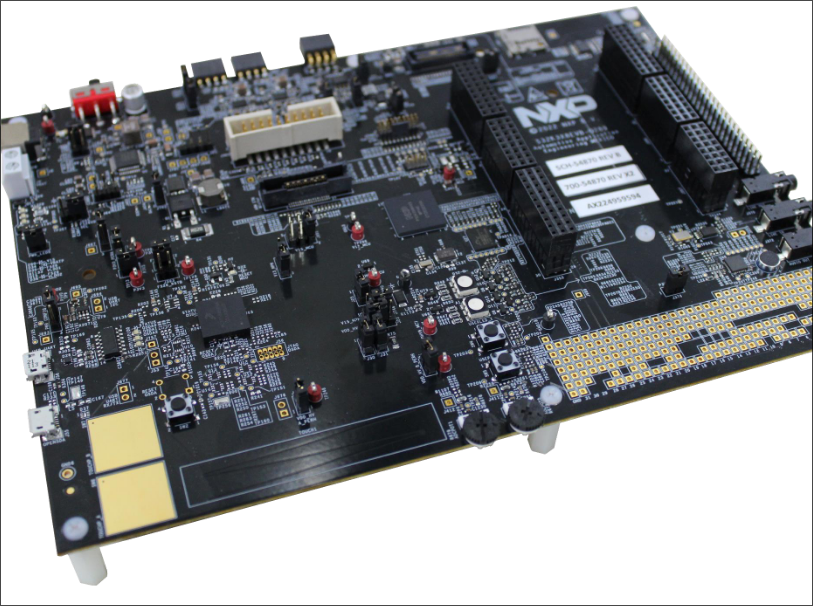
\includegraphics[width=0.7\textwidth]{chapters/figures/Board.png}
    \caption{NXP S32K3X8EVB Board}
    \label{fig:s32k3x8evbb}
\end{figure}

\subsection{Key Addresses}\label{subsec:key_addresses}

The following table lists some of the key memory-mapped addresses for the NXP S32K3X8EVB board:

\begin{itemize}
    \item {\textbf{Flash Memory}:
        \begin{itemize}
            \item { Flash0:
                \begin{itemize}
                    \item \textbf{Start Address}: 0x00400000
                    \item \textbf{Size}: 2 MB
                \end{itemize}
            }
            \item { Flash1:
                \begin{itemize}
                    \item \textbf{Start Address}: 0x00600000
                    \item \textbf{Size}: 2 MB
                \end{itemize}
            }
            \item { Flash2:
                \begin{itemize}
                    \item \textbf{Start Address}: 0x00800000
                    \item \textbf{Size}: 2 MB
                \end{itemize}
            }
            \item { Flash3:
                \begin{itemize}
                    \item \textbf{Start Address}: 0x00A00000
                    \item \textbf{Size}: 2 MB
                \end{itemize}
            }
            \item { Flash4:
                \begin{itemize}
                    \item \textbf{Start Address}: 0x10000000
                    \item \textbf{Size}: 128 KB
                \end{itemize}
            }
        \end{itemize}
        Only the first 2 MB of Flash memory has been implemented in QEMU for testing purposes.
    }
    \item {\textbf{SRAM}:
        \begin{itemize}
            \item { SRAM0:
                \begin{itemize}
                    \item \textbf{Start Address}: 0x20400000
                    \item \textbf{Size}: 256 KB
                \end{itemize}
            }
            \item { SRAM1:
                \begin{itemize}
                    \item \textbf{Start Address}: 0x20440000
                    \item \textbf{Size}: 256 KB
                \end{itemize}
            }
            \item { SRAM2:
                \begin{itemize}
                    \item \textbf{Start Address}: 0x20480000
                    \item \textbf{Size}: 256 KB
                \end{itemize}
            }
        \end{itemize}
        Only the first 256 KB of SRAM has been implemented in QEMU for testing purposes.
    }
    \item {\textbf{UART Base Addresses}:
        \begin{itemize}
            \item \textbf{UART0 Address}: 0x40328000
            \item \textbf{UART1 Address}: 0x4032C000
            \item \textbf{UART2 Address}: 0x40330000
            \item \textbf{UART3 Address}: 0x40334000
            \item \textbf{UART4 Address}: 0x40338000
            \item \textbf{UART5 Address}: 0x4033C000
            \item \textbf{UART6 Address}: 0x40340000
            \item \textbf{UART7 Address}: 0x40344000
            \item \textbf{UART8 Address}: 0x4048C000
            \item \textbf{UART9 Address}: 0x40490000
            \item \textbf{UART10 Address}: 0x40494000
            \item \textbf{UART11 Address}: 0x40498000
            \item \textbf{UART12 Address}: 0x4049C000
            \item \textbf{UART13 Address}: 0x404A0000
            \item \textbf{UART14 Address}: 0x404A4000
            \item \textbf{UART15 Address}: 0x404A8000
        \end{itemize}
        All UART peripherals have been implemented anc connected to QEMU NVIC but only UART0 has been used for testing.
    }

    \item {\textbf{SPI Base Addresses}:
        \begin{itemize}
            \item \textbf{SPI0 Address}: 0x40358000
            \item \textbf{SPI1 Address}: 0x4035C000
            \item \textbf{SPI2 Address}: 0x40360000
            \item \textbf{SPI3 Address}: 0x40364000
            \item \textbf{SPI4 Address}: 0x404BC000
            \item \textbf{SPI5 Address}: 0x404C0000
        \end{itemize}
        All SPI peripherals have been implemented anc connected to QEMU NVIC but only SPI0 has been used for testing.
    }
\end{itemize}